\chapter{Contextualización}
\label{cap:c2_context}

\definecolor{lightergray}{RGB}{247,247,247}
\definecolor{darkgreen}{RGB}{36,135,20}
\definecolor{green_comment}{RGB}{0,128,0}
\definecolor{redcell}{RGB}{238,176,176}
\definecolor{greencell}{RGB}{217,234,211}


	En este capítulo se presenta una descripción de los algoritmos de Inteligencia Artificial que se van a utilizar en el proyecto, así como sus usos y características. 
	

\section{MPI}

	Message Passing Interface\cite{barker2015message}  (MPI)  es un estándar para una biblioteca de paso de mensajes, diseñado para funcionar en una amplia variedad de arquitecturas informáticas paralelas. Permite la comunicación entre procesos, mediante el envío y recepción de mensajes. Comúnmente se utiliza en sistemas de alto rendimiento\cite{stone1990high} (HPC) y entornos informáticos paralelos para desarrollar aplicaciones paralelas escalables y eficientes.
	
	
	Al crear el entorno MPI en una aplicación, se ejecutan en paralelo varios procesos, cada uno con su correspondiente \textit{id}, también llamado \textit{rank}. El programador elige cuál va a ser el desempeño de los procesos. Por ejemplo, en el modelo \textit{Master-Worker}, el primer proceso (rank=0) generalmente, es llamado \textit{Master}, y se encarga de distribuir los datos entre los demás procesos, llamados \textit{Workers}. La Figura \ref{fig:comunicacion_mw}, muestra la comunicación entre los procesos en este modelo. El proceso \textit{Master} reparte los datos mientras que los \textit{Workers} los procesan y los devuelven.


	\begin{figure}[!h]
		\centering
		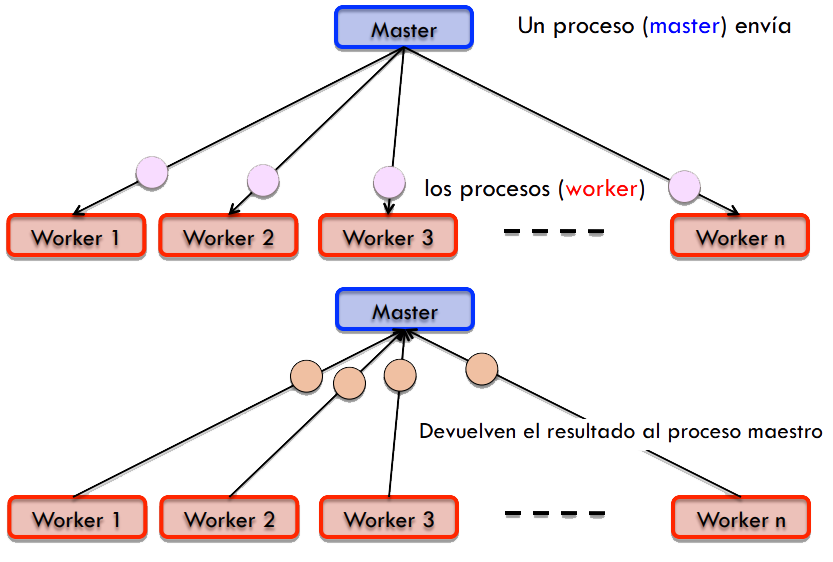
\includegraphics[width=0.65\textwidth]{images/chapter_2/mpi_1}
		\caption{Comunicación Master-Worker}
		\label{fig:comunicacion_mw}
	\end{figure}

	\newpage

	Esta técnica para paralelizar utiliza memoria distribuida, es decir, cada proceso tiene su propia memoria local. Así los procesos no tienen que preocuparse por los problemas de la memoria compartida, como la sincronización para el acceso de variables compartidas, ¡es de carrera o \textit{deadlocks}. Asimismo, la memoria compartida no es fácilmente escalable a un gran número de procesadores\cite{jjruiz2016compartida}.


	Un programa ejecutado en paralelo, donde múltiples procesos se ejecutan en el mismo programa de manera independiente, pero trabajan con diferentes conjuntos de datos. Se denomina SPMD, este modelo es comúnmente utilizado en computación de alto rendimiento y en entornos de procesamiento paralelo. La escalabilidad y eficiencia de este modelo son sus principales ventajas.

	Un proceso (\textit{Master}) contiene los datos del programa y se encarga de gestionar los mismos y repartirlos de manera eficiente. Los mensajes pueden ser:

	\begin{itemize}
		\item Síncronos: al ejecutar la función recv() el proceso receptor se queda bloqueado.
		\item Asíncrono: el receptor no se bloquea, por lo que puede adelantar código mientras espera a recibir el mensaje.
		\item Broadcast: un mensaje se envía a todos los procesos. Los emisores tienen que llamar a la misma función para recibir el mensaje.
	\end{itemize}


	\vspace{-0.2cm}

	\begin{figure}[!h]
		\centering
		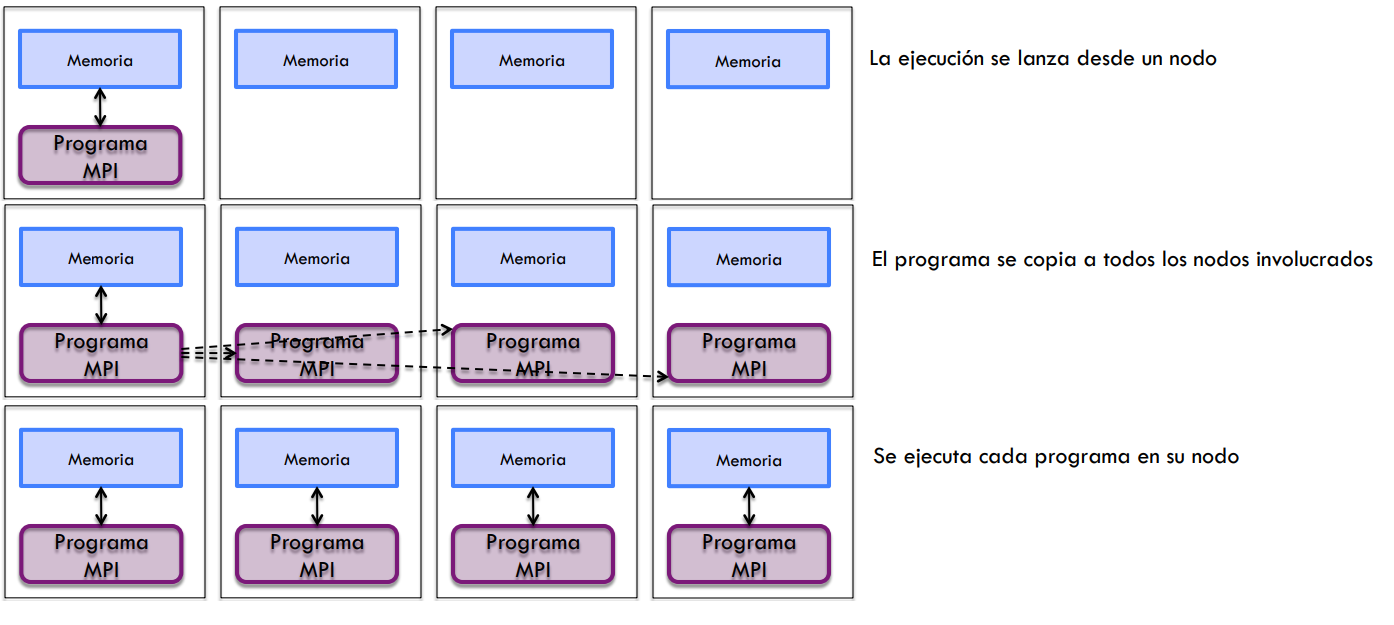
\includegraphics[width=0.9\textwidth]{images/chapter_2/mpi_2}
		\caption{Ejecución MPI}
		\label{fig:ejecucion_mpi}
	\end{figure}

	\vspace{-0.2cm}
	
	Un programa MPI (ver Figura \ref{fig:ejecucion_mpi}), comparte el mismo código para todos los procesos ejecutados. Un proceso lee el conjunto de datos y los carga en su memoria, para luego dividirlos y enviarlos a los procesos disponibles. Una vez repartido el \textit{dataset} se ejecutan en paralelo y procesan los datos recibidos. Cuando un proceso finaliza el procesado de los datos, envía los datos procesados al proceso correspondiente. La Figura \ref{fig:esquema_mpi} representa en código esta idea.
	
	\vspace{-0.1cm}

	\begin{figure}[!h]
		\lstset{language=python, 
			language=python,
			breaklines=true,
			basicstyle=\footnotesize\ttfamily,
			backgroundcolor=\color{lightergray},
			keywordstyle=\color{blue}, % Keywords will be blue
			commentstyle=\color{green!60!black}, % Comments will be green
			stringstyle=\color{purple}, % Strings will be purple
			numbers=left, % Line numbers will appear on the left
			numberstyle=\tiny\color{gray}, % Line numbers will be small and gray
			frame=single,}
		
		\begin{lstlisting}[frame=single]
 from mpi4py import MPI 
 # Al importar la biblioteca en Python se genera el entorno.

 comm = MPI.COMM_WORLD     	# Comunicador
 status = MPI.Status()   	# Status
 myrank = comm.Get_rank() 	# id de cada proceso
 numProc = comm.Get_size() 	# Numero de procesadores

 if myrank==0:           	# Master
    # Carga el conjunto de datos. Los divide y envia.
    # Recibe todos los datos procesados.
 else:                   	# Workers
    # Recibe el subconjunto de datos que le asigna el Master.
    # Procesa los datos.
    # Envia los datos procesados.
		\end{lstlisting}
		\caption{Esquema básico para ejecutar un programa MPI en Python}
		\label{fig:esquema_mpi}
	\end{figure}
	
	\newpage

\section{Aprendizaje por Refuerzo}

	Reinforcement Learning (RL, por sus siglas en inglés), en español, Aprendizaje por Refuerzo, es un tipo de aprendizaje automático donde el agente aprende en base a las decisiones tomadas al interactuar con el entorno. El agente aprende a cumplir un objetivo en un entorno ejecutando un determinado número de acciones. Este tipo de algoritmos no requiere de entradas etiquetadas como en el aprendizaje supervisado, sino que recibe una retroalimentación, \textit{feedback} en inglés (recompensas o castigos), al realizar acciones en los estados. Aprendiendo con prueba y error, el agente explora el entorno para almacenar las mejores acciones para cada estado. 

	\begin{flushleft}
		Los componentes esenciales del algoritmo son los siguientes:
	\end{flushleft}
	\begin{itemize}
		\item Agente, que interactúa con el entorno y aprende de él, ejecutando sus acciones. 
		\item Entorno, con el cual el agente interactúa. Responde a las acciones tomadas por el agente y provee el \textit{feedback}.
		\item Conjunto de acciones o decisiones que el agente puede realizar.
		\item Estados, son las configuraciones que el entorno puede tomar.
		\item Feedback, recompensas o castigos del entorno al realizar una acción en un estado.		
		\item Condición de finalización. La cual abarca desde encontrar la función óptima, hasta realizar un número de acciones 
	\end{itemize}


	\subsection{Algoritmo Q-Learning} 
		El algoritmo Q-Learning es una mezcla entre programación dinámica y Monte Carlo \cite{wang2012monte}. Es el más básico de entre los algoritmos de aprendizaje por refuerzo. Se usa para encontrar la mejor política de selección de acciones para un proceso de Decisión de Markov Determinado (MDP, por sus siglas en inglés) \cite{garcia2013markov}. 
		
		El procedimiento se realiza actualizando iterativamente las estimaciones de calidad de realizar dicha acción en el estado actual, conocido como valor-Q. Se suele representar en forma de matriz \textit{Q(S,A)}, guardando los valores-Q de las acciones en los estados. Este valor representa cómo de buena es la acción a realizar en un estado después de realizar una etapa de entrenamiento. Para ello, la Figura \ref{fig:qvalue} muestra la fórmula para actualizar los valores, para cada acción tomada por el agente.
				
		
		\begin{figure}[!h]				
		\begin{flushleft}
		\begin{mdframed}[roundcorner=5pt]
			\[
			Q(S,A) = (1 - \alpha) Q(S,A) + \alpha \left( R(S,A) + \max_{i} \{ Q(S',A_i) \} \right)
			\]
			\begin{itemize}
				\item \( Q(S,A) \) ← Es el valor-Q de ejecutar la acción \( A \) en el estado \( S \).
				\item \( R(S,A) \) ← Es la recompensa obtenida al ejecutar la acción \( A \) en el estado \( S \).
				\item \( \alpha \) ← Tasa de aprendizaje. Controla cuánta importancia le da a la nueva información frente a la antigua.
				\item \( \gamma \) ← Factor de descuento. Determina la importancia de futuras recompensas comparadas con las recompensas inmediatas.
				\item \( max_{i}(Q(S',A_i)) \) : Es el valor máximo obtenible de realizar las posibles acciones en el estado siguiente.
			\end{itemize}
		\end{mdframed}		
		\end{flushleft}
		\caption{Cálculo del Q-Value de un estado y acción}	
		\label{fig:qvalue}
		\end{figure}
		
		
		El agente toma las decisiones de ejecutar una acción dependiendo del hiper-parámetro $\epsilon$  con valores entre [0,1]. Con un número aleatorio (en el mismo intervalo) calcula la probabilidad de ejecutar la mejor acción aprendida hasta el momento, o una acción aleatoria entre las disponibles. Si el valor es alto, casi siempre se ejecutará la mejor acción aprendida hasta el momento, y es posible que no aprenda otras formas de alcanzar el objetivo.
		
		%\newpage
		
		Este algoritmo se ha aplicado en muchos dominios, como puede ser videojuegos de Atari \cite{mnih2013playing}, robótica o problemas de optimización. Sin embargo sufre cuando el entorno tiene muchos estados, ya que la complejidad espacial aumenta considerablemente, y no es práctico tener las dos matrices. Por eso se diseñó el algoritmo DQN que usa una red neuronal. Así eliminamos la maldición de dimensionalidad \cite{kuo2005lifting}, problemas que surgen con el exceso de variables independientes en un dataset. En este algoritmo, el problema es el elevado número de estados que el agente ha de recorrer.\\
		
	\subsection{Deep Q-Network (DQN)}
		Deido a los problemas de escalabilidad mencionados anteriormente, se desarrolló el algoritmo de Redes Neuronales Profundas (DQN,por sus siglas en inglés). Este algoritmo combina redes neuronales con la base de aprendizaje por refuerzo, eliminando así la Q-Table.
		
		La estructura de la red neuronal depende del entorno del problema. Los valores de la capa oculta se pueden modificar dependiendo de las necesidades del programador, pero la capa de entrada y salida depende del problema. La entrada se adapta para recibir un estado del entorno, y la salida tendrá tantos nodos como las acciones del agente. 
		
		El problema a realizar tendrá dos redes neuronales, una del estado actual y otra de anticipo, es decir, el siguiente estado. Esto sirve para ayudar a tener más contexto del estado actual, pues con una sola imagen (estado del juego), la información del estado puede variar considerablemente. En la fase de entrenamiento se realizan varios episodios, que consisten en ejecuciones hasta que se de una condición de finalización. Además de ejecutar repeticiones de estados guardados anteriormente (replay buffer). En este algoritmo se usan tres hiper-parámetros: 
		\begin{enumerate}
			\item Gamma, factor de descuento. Utilizado para saber cuanto resta a la recompensa adquirida al realizar una acción en un estado.
			\item Epsilon, tasa de exploración. Probabilidad utilizada para ejecutar una acción aleatoria o la mejor hasta el momento.
			\item Learning rate, tasa de aprendizaje. Para la propagación hacia atrás de las redes neuronales. Ensencialmente, mide cuánto cambian los pesos de los nodos al tener un fallo.
		\end{enumerate}	
		
		
		
		En este trabajo, el entorno del problema será el juego de la empresa \textit{Namco}, la versión de \textit{Atari 2600}, \textit{Pac-Man} (ver Figura \ref{fig:pacman}). El juego consiste en recolectar todas las monedas del laberinto sin ser comido por un fantasma. Implementamos el juego -desde cero- para moldear a nuestro gusto la implementación y que el algoritmo DQN sea más eficiente y sencillo. En el capítulo \ref{cap:c3_implementaciones}, diseño e implementaciones, se desarrolla en profundidad.
		
		\begin{figure}[!h]			
			\centering
			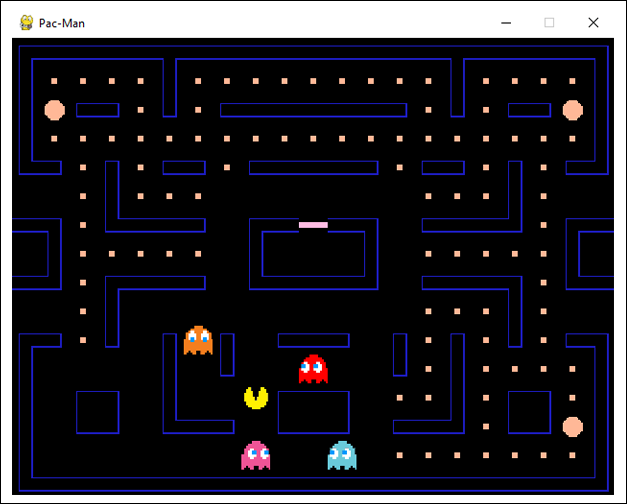
\includegraphics[width=0.50\textwidth]{images/chapter_2/pacman}	
			\caption{Juego Pac-Man version Atari 2600}
			\label{fig:pacman}
		\end{figure}
		
	
		\newpage

\section{Aprendizaje No-Supervisado}

	Los métodos no supervisados (unsupervised methods, en inglés) son algoritmos de aprendizaje automático que basan su proceso en un entrenamiento con datos sin etiquetar. Es decir, a priori, no se conoce ningún valor objetivo, ya sea categórico o numérico. 
	
	La meta de este aprendizaje es encontrar patrones o estructuras en los datos proporcionados. Estos algoritmos son útiles en escenarios en los cuales hay escasez de datos etiquetados o no están disponibles.
	
	Hay muchos tipos de técnicas de aprendizaje no supervisado, como, entre otros, la detección de anomalías, reducción de dimensionalidad o \textit{clustering}. En este proyecto vamos a reducir el tiempo de ejecución de las técnicas de \textit{clustering} que se encargan de agrupar individuos, basándose en alguna medida de similitud. Como no es aprendizaje supervisado, no disponemos de información categorizada previamente, por lo que hay que calcular el número óptimo de \textit{clusters}. Para ello, cual medidas ya estudiadas como el diagrama de ``codo'', cuyo valor óptimo de clusters se calcula visualmente, cuando empieza a crearse un codo (la diferencia con el número anterior no es tan pronunciada como en puntos anteriores). Hay otros coeficientes que calculan la optimalidad con algoritmos, como el coeficiente de Davies-Bouldin, cuyo valor mínimo indica el número óptimo de clusters, o el coeficiente de Silhouette, siendo similar al anterior, pero con el valor máximo. Se pueden apreciar los diferentes coeficientes en la Figura \ref{fig:coeficientes}. 


	\begin{figure}[!h]
		\centering
		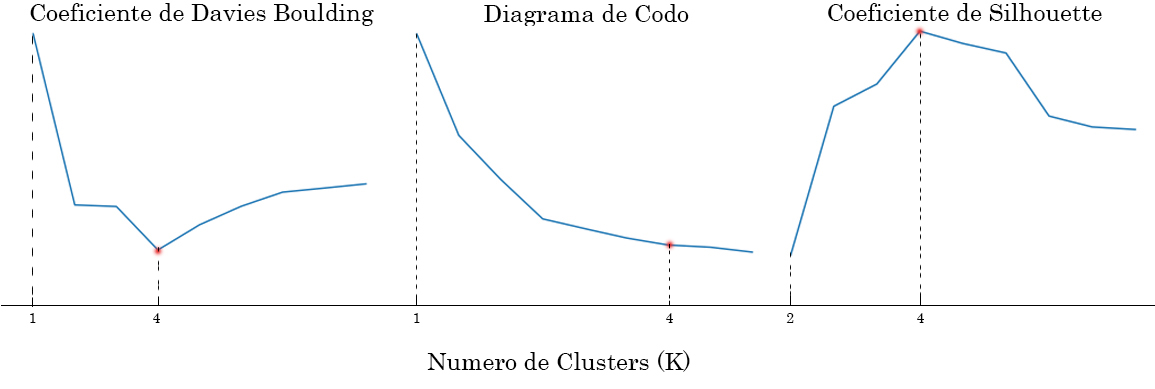
\includegraphics[width=0.90\textwidth]{images/chapter_2/ap_nosup_diagramas}
		\caption{Coeficientes}
		\label{fig:coeficientes}
	\end{figure}
	
	\newpage


	Los llamados métodos jerárquicos \cite{ackermann2014analysis} tienen por objetivo agrupar \textit{clusters} para formar uno nuevo o bien separar alguno ya existente para dar origen a otros dos, de tal forma que, si sucesivamente se va efectuando este proceso de aglomeración, se minimice alguna distancia o bien se maximice alguna medida de similitud.

	\subsection{Clustering jerárquico aglomerativo}

		Este algoritmo usa una matriz para realizar la agrupación de los individuos. Comienza teniendo N clusters, uno por cada individuo de la población. La matriz se representa por las filas, es decir, la fila i-ésima representa el cluster i-ésimo. La matriz se rellena con las distancias entre los \textit{clusters}, por lo que la celda (i,j) representa la distancia entre el cluster \textit{i} y el \textit{j}.  
		
		En cada iteración, se busca en la matriz la distancia mínima, y se juntan los \textit{clusters} que representan la fila \textit{i} con la columna \textit{j}. La matriz se actualiza, eliminando la fila y la columna con mayor índice (entre \textit{i},\textit{j}), y actualizando la fila y columna de menor índice. Este proceso se repite hasta que solo haya un \textit{cluster}. Las distancias entre \textit{clusters} pueden ser:
		\begin{itemize}
		\vspace{-0.25cm}
		\item Centroides: cada cluster tiene un centro.
		\vspace{-0.25cm}
		\item Enlace simple o compuesto: la distancia entre \textit{clusters} viene dada por la menor o mayor distancia, respectivamente, entre los individuos que representan cada \textit{cluster}.
		\vspace{-0.30cm}
		\end{itemize}



		\begin{algorithm}[!h]
			\caption{Jerárquico Aglomerativo}
			\KwData{poblacion, C // Número de clusters deseados}
			\KwResult{agrupacion // Clusters para cada individuo de la población}
			D := init() // Inicializar la matriz de distancias\\
			\While{number of rows in $matrix$ $> C$}{
				// Recorrer la matriz en búsqueda del menor valor (i, j)\\
				busqueda\_min(poblacion)
				// Agrupar los cluster (i, j)\\
				agrupar\_clusters(poblacion, i, j);
				// Eliminar la fila y columna de mayor índice\\
				eliminar\_cluster(poblacion, max(i, j))		
				
				// Calcular nuevas distancias al cluster agrupado (i)
				nuevas\_distancias(poblacion, min(i, j))
			}
			
		\end{algorithm}
		\vspace{-0.20cm}

		\noindent La complejidad en los enlaces simple y completo tienen un coste cúbico O(\(N^{3}\)), al tener que comparar todos los individuos uno a uno entre dos cluster.
		
		\newpage


		Al finalizar la ejecución se puede representar la agrupación mediante un dendrograma \cite{espinoza2012using}, y comprobar el número óptimo de \textit{clusters} para la población calculada. Sin embargo, no es igual de preciso que los coeficientes mencionados anteriormente. (ver Figura \ref{fig:dendograma})
		
		\begin{figure}[!h]
			\centering
			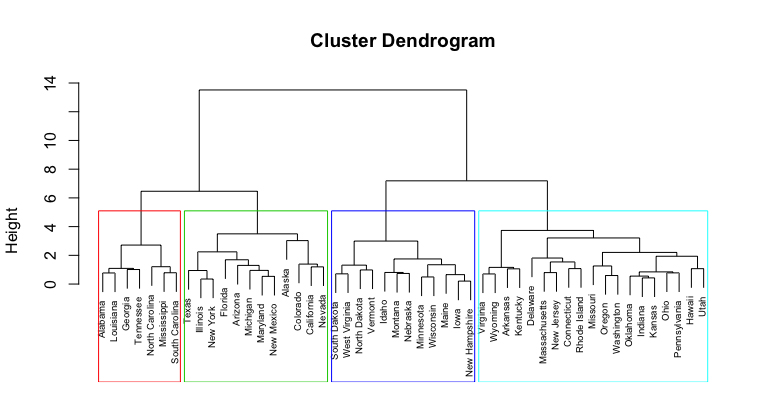
\includegraphics[width=0.9\textwidth]{images/chapter_2/dendograma}
			\caption{Dendograma}
			\label{fig:dendograma}
		\end{figure}


	\subsection{Clustering basado en particiones: K-Medias}

		La meta de este algoritmo es particionar la población inicial en \textit{K} clusters, cada individuo se agrupa con el \textit{cluster} más próximo. Para ello se busca minimizar el sumatorio de distancias entre los individuos y el centroide de su \textit{cluster}. 
		
		
		\begin{algorithm}[!h]
			\caption{K-Medias}
			\KwData{poblacion, K}
			\KwResult{agrupacion}
			centrosNuevos := init(K) // Inicializar los centros de manera aleatoria\\
			
			\Repeat{$centros$ $!= centrosNuevos$}
			{
				centros := centrosNuevos\\
				agrupacion := asignar(poblacion)\\
				centrosNuevos := calculaCentros(poblacion, asignacion)
			}
			
			
			\Return $agrupacion$\;
		\end{algorithm}
		
		Sin embargo, hay que tener en cuenta que la inicialización de los centros es estocástica, por lo que el algoritmo puede converger en un óptimo local. Por eso es importante repetir el algoritmo varias veces para encontrar el óptimo general. La Figura \ref{fig:kmediasBusqueda} muestra una ejemplo de ejecución de este algoritmo. En este caso, se ejecuta varias veces el algoritmo, para ver las posibles asignaciones. El intento con menor valor del sumatorio de distancias de individuos y su cluster asignado, es la mejor asignación entre los intentos ejecutados.



		% TODO CAMBIAR IMAGEN
		\begin{figure}[!h]
			\centering
			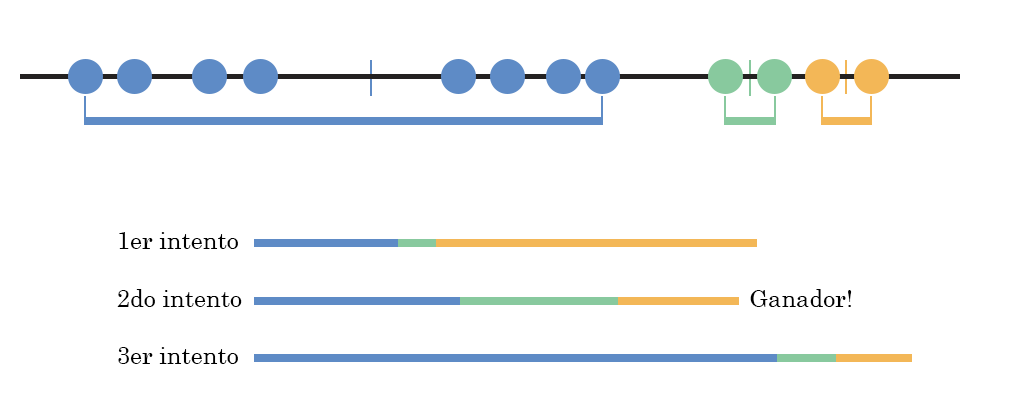
\includegraphics[width=1\textwidth]{images/chapter_2/kmedias}
			\caption{KMedias - Búsqueda}
			\label{fig:kmediasBusqueda}
		\end{figure}


\section{Aprendizaje Supervisado}
	Al contrario que el apartado anterior, este tipo de aprendizaje automático, es entrenado con un \textit{dataset} categorizado con su salida correcta. El algoritmo aprende de este conjunto para hacer predicciones sobre unos datos desconocidos.
	
	El objetivo de este algoritmo es aprender la función que mapea las variables de entrada en las categorías correctas de salida. Para ello, ajusta los parámetros con técnicas de optimización iterativas para minimizar el error en sus predicciones.
	
	Los ejemplos más comunes son la clasificación, para dividir la población en categorías según unos parámetros, y regresión, que encuentra las correlaciones entre las variables dependientes e independientes.


	\subsection{K-Vecinos más Cercanos - KNN}

		KNN es un algoritmo simple pero potente, es muy efectivo para tareas de clasificación y regresión. Se basa en la idea de que los puntos de datos similares tienden a agruparse en el espacio de características. Pertenece al paradigma de aprendizaje perezoso o basado en instancias.
		
		\begin{itemize}
			\item Perezoso: no calcula ningún modelo y demora todos los cálculos hasta el momento en que se le presenta un ejemplo nuevo.			
			\item Basado en instancias: usa todos los individuos disponibles y ante un ejemplo nuevo recupera los más relevantes para componer la solución.	
		\end{itemize}
		
		No hay una forma de determinar el mejor valor para K, de forma que hay que probar con varias ejecuciones. Valores pequeños de K crea sonido, provocando que inicialmente se categorice con un cluster no tan idoneo, y a la larga se categoricen muchos de forma incorrecta. Valores grandes con pocos datos favorece a los \textit{clusters} con mas individuos. Un valor diferente de K puede cambiar la categoría de un individuo. En la Figura \ref{fig:knn} se puede apreciar el proceso de asignación de un cluster a un nuevo individuo. Como se puede ver con los círculos que delimitan los K vecinos más cercanos, si variamos K, la asignación del nuevo individuo puede cambiar.

		\begin{algorithm}
			\caption{KNN}
			\KwData{poblacion, etiquetas, poblacionPred}
			\KwResult{agrupacion // Clusters para cada individuo de la población}
			agrupacion := $\emptyset$\\
			\For{each individuo $ind$ in $poblacionPred$}{
				// Recorrer toda la población guardando los K individuos más cercanos\\
				vecinos := recorrer\_poblacion(poblacion, individuo)\\
				// Clasificar según los K vecinos\\
				cluster := clasificar\_individuo(vecinos)\\
				agrupacion.append(cluster, etiquetas)
			}
			\Return $agrupacion$
		\end{algorithm}
		
		La distancia entre individuos más usada es la Euclídea, pero requiere más tiempo al aplicar potencias y raíces cuadradas en su cálculo. La distancia Manhattan es más rápida, pero menos precisa.



		%\begin{figure}[!h]
		%	\centering
		%	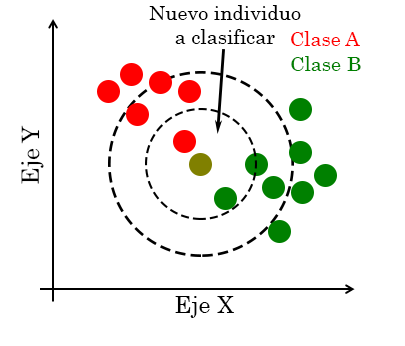
\includegraphics[width=0.5\textwidth]{images/chapter_2/knn}
		%	\caption{KNN}
		%	\label{fig:knn}
		%\end{figure}
		
		
		\begin{figure}[!h]
			\centering
			
			
			\begin{subfigure}[t]{0.4\textwidth}
				\centering
				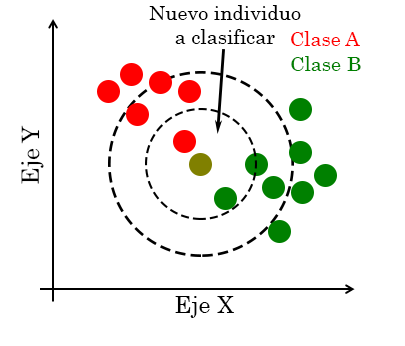
\includegraphics[width=\textwidth]{images/chapter_2/knn}
				\caption{KNN}
				\label{fig:knn}
			\end{subfigure}
			\hfill
			\begin{subfigure}[t]{0.5\textwidth}
				\centering
				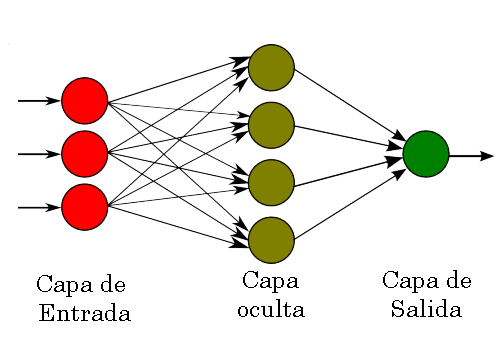
\includegraphics[width=\textwidth]{images/chapter_2/redneu}
				\caption{Red Neuronal}
				\label{fig:redneu}
			\end{subfigure}
			
			\caption{Aprendizaje Supervisado}
			\label{fig:aprendizajeSupervisado}
		\end{figure}

	\subsection{Redes Neuronales}

		Las redes neuronales son un modelo computacional inspirado en el funcionamiento y estructura de las neuronas del cerebro humano. Consiste en capas de nodos interconectados, llamadas neuronas artificiales. La estructura del modelo se muestra en la Figura \ref{fig:redneu}. En este modelo se aprecian:


		\begin{itemize}
			\item Capa de entrada, en la cual, habrá tantas neuronas como variables de entrada tenga el modelo de predicción.
			\vspace{-0.4cm} 
			\item Capa oculta, representada con una o más capas internas. Cada una contiene un número determinado de neuronas.
			\vspace{-0.4cm}	
			\item Capa de salida. Como en la entrada, tendrá un número de neuronas relacionadas con las variables de salida.
		\end{itemize}
		
		\vspace{-0.2cm}
		
		Se ha demostrado que tiene un rendimiento notable en muchas tareas, como el reconocimiento de imágenes o procesamiento de lenguaje natural. Aprenden patrones complejos al someterse a un entrenamiento específico con un amplio \textit{dataset} categorizado.	
		
		%\begin{figure}[!h]
		%	\centering
		%	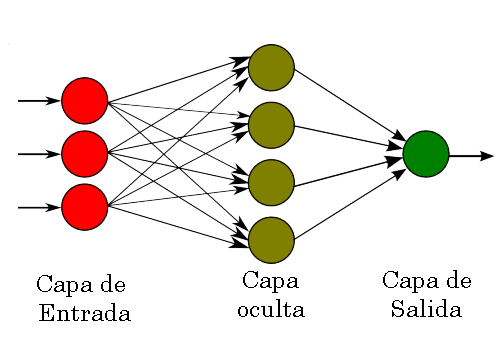
\includegraphics[width=0.5\textwidth]{images/chapter_2/redneu}
		%	\caption{Red Neuronal}
		%	\label{fig:redneu}
		%\end{figure}
		
		En el proceso de entrenamiento aprende a realizar una tarea específica ajustando los parámetros internos (pesos en las conexiones), gracias al \textit{dataset} proporcionado. Normalmente, este ajuste se lleva a cabo con algoritmos de optimización como descenso de gradiente, donde se comparan las predicciones del modelo con la categoría correcta, y se actualizan los parámetros del modelo con un método de propagación hacia atrás, \textit{backpropagation} en inglés. Estos valores se actualizan dependiendo del error cometido y la tasa de aprendizaje proporcionada al modelo.



		\begin{algorithm}
			\caption{Red Neuronal}
			\KwData{entrenamiento, etiquetas, evaluacion // Individuos sin categorizar\\
					\Indp \Indp repeticiones, capas // Tam. entrada, oculta, salida}
			\KwResult{pesos // Opcionalmente, devolver los pesos de la red}
			pesos := init() // Inicializar los pesos de manera aleatoria\\
			\For{$rep \leftarrow 0$ \KwTo $repeticiones$}{
				cont := 0
				\For{each $ind$ in $entrenamiento$}{
					// Suma el valor recibido de la capa anterior multiplicada por los pesos de la capa actual con la siguiente. Así se determina la importancia de conexión entre las neuronas. \\
					// Con el valor calculado se aplica a una función de activación y se pasa a la siguiente capa hasta llegar a la salida.\\			
					predicion := \textbf{forward(pesos, ind)}\\
					// El valor predicho calculado en la salida es comparado con la etiqueta, y se calcula el error. Este error se manda para atrás actualizando los pesos. Se suma la multiplicación del valor predicho en cada capa con la tasa de aprendizaje y el error.\\			
					\textbf{backpropagation(pesos, predicion, etiqueta[cont])}
					cont++
				}
			}
			
			
			\Return $agrupacion$
		\end{algorithm}



		%\vspace{0.2cm}
		
		%\begin{figure}[!h]
		%	\centering
		%	
		%	
		%	\begin{subfigure}[t]{0.33\textwidth}
		%		\centering
		%		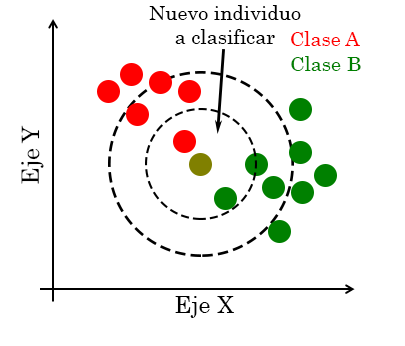
\includegraphics[width=\textwidth]{images/chapter_2/knn}
		%		\caption{KNN}
		%		\label{fig:knn}
		%	\end{subfigure}
		%	\hfill
		%	\begin{subfigure}[t]{0.48\textwidth}
		%		\centering
		%		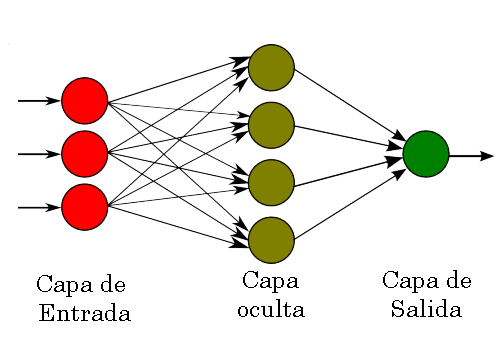
\includegraphics[width=\textwidth]{images/chapter_2/redneu}
		%		\caption{Red Neuronal}
		%		\label{fig:redneu}
		%	\end{subfigure}
		%	
		%	\caption{Aprendizaje Supervisado}
		%	\label{fig:aprendizajeSupervisado}
		%\end{figure}
		









\section{Programación Evolutiva}


	La programación evolutiva es una técnica de optimización inspirada en la teoría de la evolución biológica. Se basa en el concepto de selección natural y evolución de las poblaciones para encontrar soluciones a problemas complejos. 
	
	La población está compuesta por individuos, que pueden ser representados con arrays de números reales, binarios o un árbol, en programación genética. Los individuos tienen un cromosoma, que a su vez tiene uno o varios genes, con uno o más alelos. Esta población es sometida a métodos de selección, mutación y evaluación para, con el paso de las generaciones, maximizar o minimizar un valor \textit{fitness}.
	
	Esta técnica es muy útil para problemas de optimización donde los métodos tradicionales son no proporcionan el rendimiento deseado.  Se han aplicado a varios dominios, como por ejemplo la bioinformática o robótica \cite{contreras2015mobile}.


	\begin{figure}[!h]
		\centering
		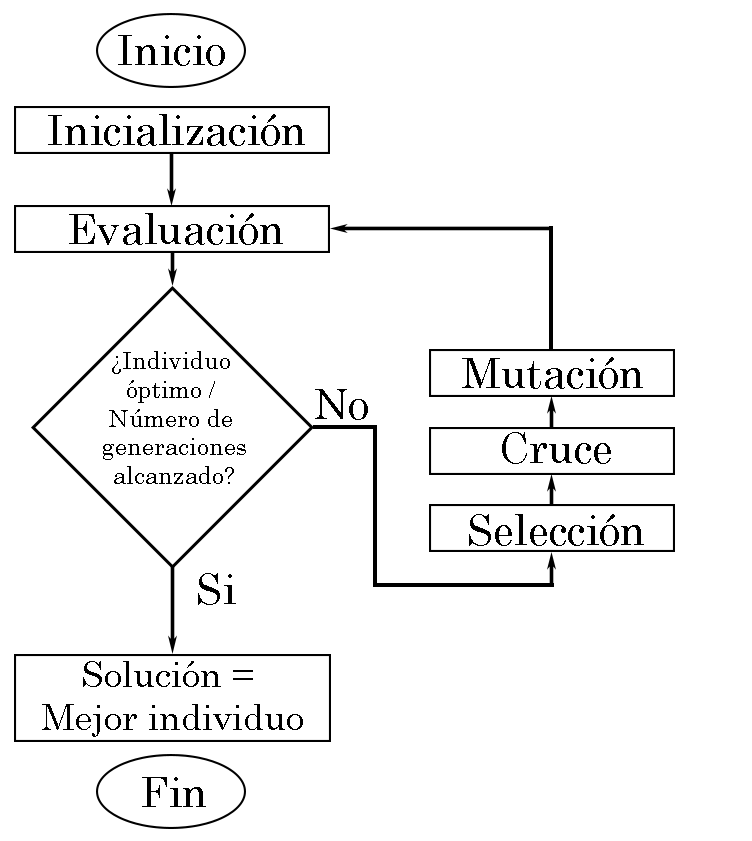
\includegraphics[width=0.45\textwidth]{images/chapter_2/AG}
		\caption{Algoritmo Evolutivo}
		\label{fig:AG}
	\end{figure}




%Aquí comienza la descripción del trabajo realizado. Se deben incluir tantos capítulos como sea necesario para describir de la manera más completa posible el trabajo que se ha llevado a cabo. Como muestra la figura \ref{fig:sampleImage}, está todo por hacer.
%
%\begin{figure}[h]
%	\centering
%	\includegraphics[width = 0.5\textwidth]{Imagenes/Vectorial/Todo.pdf}
%	\caption{Ejemplo de imagen}
%	\label{fig:sampleImage}
%\end{figure}
%
%Si te sirve de utilidad,  puedes incluir tablas para mostrar resultados, tal como se ve en la tabla \ref{tab:sampleTable}.
%
%
%\begin{table}
%	\centering
%	\begin{tabular}{c|c|c}
%		\textbf{Col 1} & \textbf{Col 2} & \textbf{Col 3} \\
%		\hline\hline
%		3 & 3.01 & 3.50\\
%		6 & 2.12 & 4.40\\
%		1 & 3.79 & 5.00\\
%		2 & 4.88 & 5.30\\
%		4 & 3.50 & 2.90\\
%		5 & 7.40 & 4.70\\
%		\hline
%	\end{tabular}
%	\caption{Tabla de ejemplo}
%	\label{tab:sampleTable}
%\end{table}
